\documentclass[runningheads]{llncs}
\usepackage{amsmath,amssymb}
\usepackage{graphicx}
\usepackage{booktabs}
\usepackage{multirow}
\usepackage{url}
\usepackage{hyperref}
\usepackage{xcolor}

\begin{document}

\title{IntentAgent: Intent-Aware Progressive Intelligent Retrieval\\for Retrieval-Augmented Generation}

\author{Author Name}
\institute{Institution}

\maketitle

\begin{abstract}
Existing retrieval-augmented generation (RAG) systems apply a uniform retrieval strategy regardless of query intent, overlooking the decisive influence that intent exerts on the choice of retrieval path. This paper proposes IntentAgent, an intent-aware progressive intelligent retrieval framework for RAG whose central thesis is that query intent should be treated as a first-class citizen in retrieval strategy selection. IntentAgent evolves through three stages along a controllability--adaptivity spectrum. In the first stage, intent classification and static routing, the system defines six query-intent categories (factual, analytical, comparative, multi-hop, exploratory, and follow-up), builds a cascaded dual-path classifier that combines an LLM primary path with a regex-based fallback, and routes each intent label to a differentiated retrieval strategy through a deterministic mapping table. In the second stage, dynamic tool orchestration, the retrieval process is modeled as a five-node cyclic directed state graph in which the LLM autonomously selects and composes retrieval tools following a reason-act protocol; a dual-mode reflection mechanism combining heuristic scoring with LLM semantic critique, together with a strategy fallback ladder, realizes Reflexion-style self-correction, while a CrossEncoder reranker provides semantic-level result refinement. In the third stage, experiential memory augmentation, an intent-bucketed persistent store follows a recall--inject--persist closed loop in which failure lessons preferentially adopt semantic reflection text, endowing the system with cross-session self-improvement. Experiments on HotpotQA, 2WikiMultiHopQA, and MuSiQue with Gemma4-12B, Qwen3-8B, and Qwen3-32B backbones show that IntentAgent surpasses all baseline methods on the majority of datasets, including the previously strongest baseline HippoRAG2, and substantially outperforms the remaining text-based, graph-based, and hybrid retrieval methods. Ablation studies confirm that intent classification is the core contributing component (EM drops by 13.3\%--16.8\% upon removal), followed by dynamic orchestration and the reflection loop. IntentAgent also achieves the highest faithfulness and answer relevancy scores, validating the substantial advantage of intent-aware retrieval in reducing hallucination and improving semantic relevance.

\noindent\textit{Keywords:} Retrieval-augmented generation, intent-aware retrieval, experiential memory, agent
\end{abstract}

\section{Introduction}

Retrieval-augmented generation (RAG) augments large language models with external knowledge retrieval at inference time and has become the dominant paradigm for mitigating hallucination and improving factual accuracy~\cite{ref1}. A typical RAG system follows a retrieve-read-generate pipeline: given a user query, it first retrieves relevant passages from a knowledge base and then feeds them as context to an LLM for answer generation~\cite{ref2}.

Existing RAG systems, however, share an implicit and restrictive assumption at the retrieval stage, which we term the \emph{strategy homogeneity assumption}: the same retrieval procedure is applied irrespective of query intent, typically a single-pass vector similarity search. This assumption breaks down in the face of real-world query diversity. Consider three representative query types. A factual query such as ``Who invented the World Wide Web?'' requires only a single vector lookup to locate the answer passage. A multi-hop reasoning query such as ``How did Einstein's alma mater influence the development of quantum mechanics?'' demands bridging inference across multiple entities, and a single retrieval pass rarely covers the complete evidence chain. A comparative query such as ``Compare the performance of BERT and GPT on text classification'' requires parallel retrieval of information about both entities followed by structured comparison.

The optimal retrieval paths for these three query types differ markedly. Routing a multi-hop reasoning query into a single-pass vector retrieval pipeline often leads to incomplete or missing evidence, whereas applying a complex multi-hop strategy to a simple factual query introduces unnecessary latency and computational overhead.

\begin{figure*}[htbp]
\centering
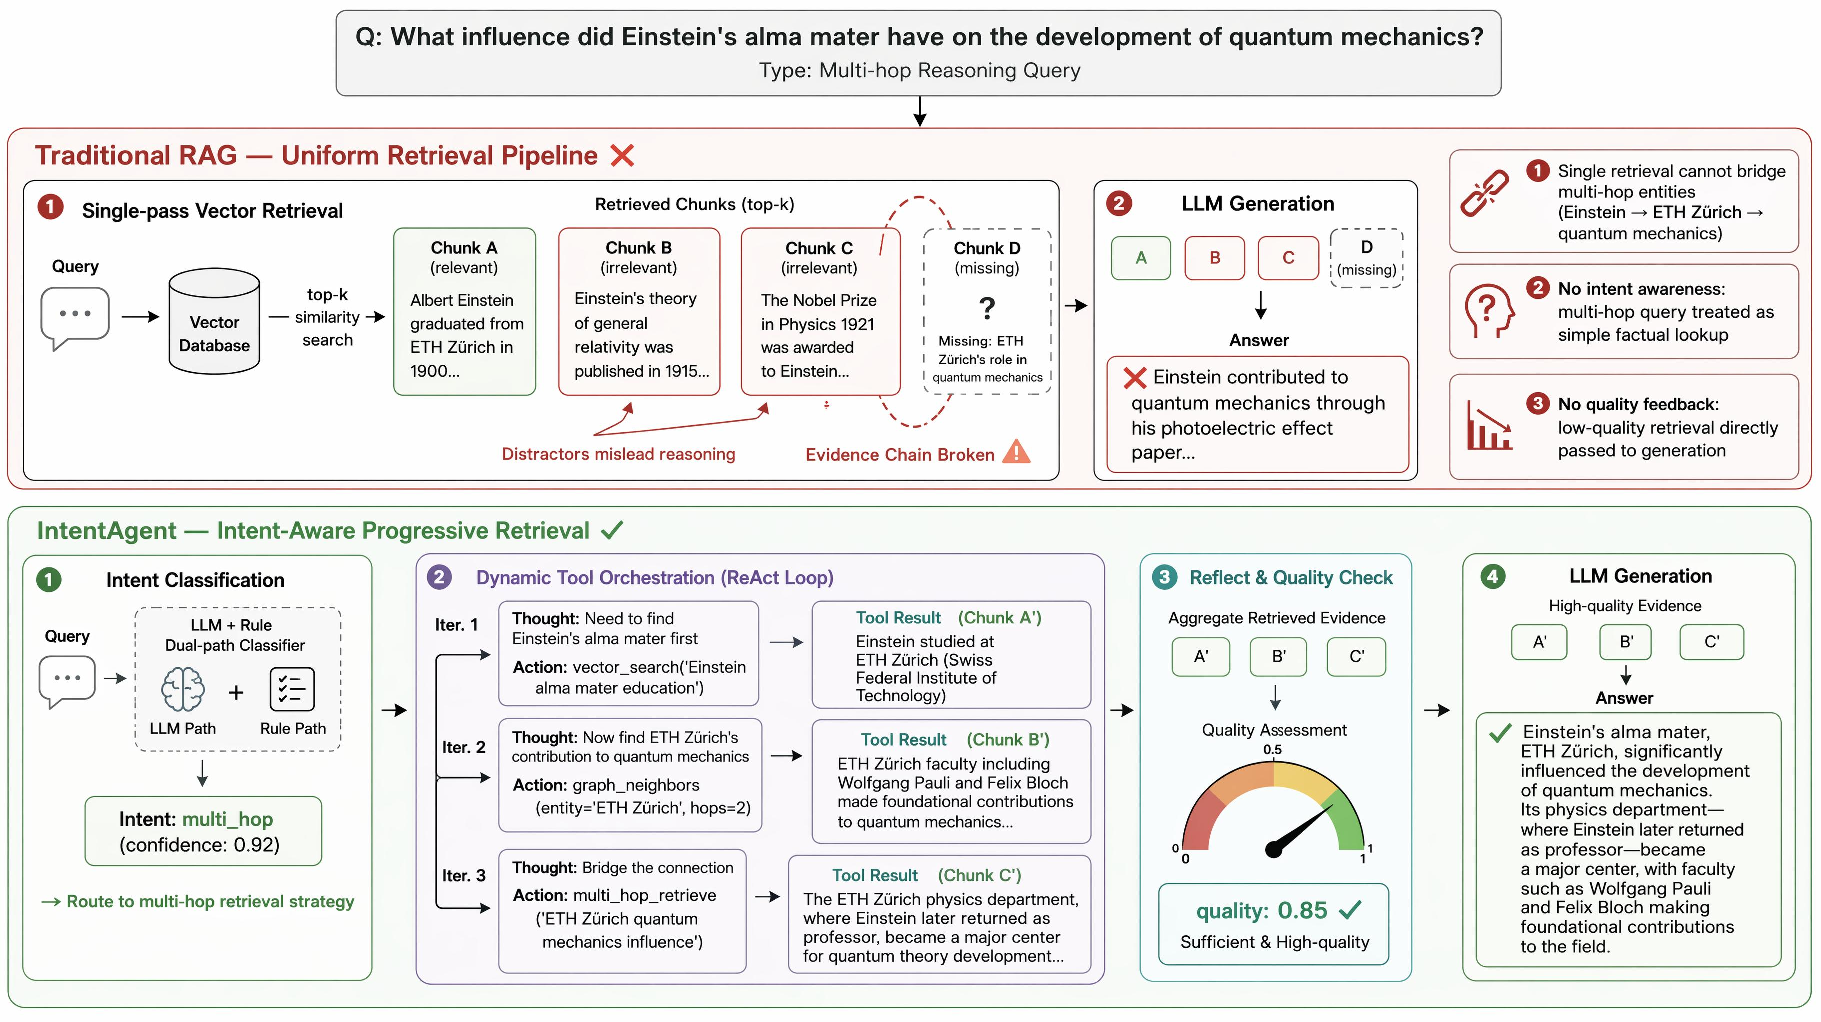
\includegraphics[width=\textwidth]{figures/figure1.pdf}
\caption{Comparison between conventional RAG and IntentAgent. Using the multi-hop query ``How did Einstein's alma mater influence the development of quantum mechanics?'' as an example, the upper half illustrates how conventional RAG suffers from evidence chain breakage and distractor interference due to strategy homogeneity, while the lower half shows how IntentAgent assembles the complete evidence chain through intent-aware progressive retrieval.}
\label{fig:comparison}
\end{figure*}

Although a variety of improvements at the retrieval-mechanism level have emerged in recent years, including the hierarchical summary tree of RAPTOR~\cite{ref23}, the community-based summarization of GraphRAG~\cite{ref27}, the dual-level retrieval of LightRAG~\cite{ref26}, the hippocampal memory indexing of HippoRAG~\cite{ref28} and HippoRAG2, and the reasoning-guided navigation on knowledge graphs in TOG~\cite{ref24}, these methods innovate on the retrieval back-end yet none of them addresses strategy homogeneity at the strategy-selection level: the retrieval strategy is fixed by the system architecture at deployment time, the same retrieval pipeline fires for every query, and query intent has no influence on strategy routing. Under this framework, factual queries incur unnecessary latency because a costly multi-hop graph expansion is invoked; multi-hop reasoning queries suffer from evidence chain breakage because cross-entity graph expansion is unavailable; comparative queries receive only one-sided information because parallel sub-retrieval is absent. The root cause lies not in the retrieval mechanism itself but in the indifference of the strategy-selection logic to query intent. Intent-aware differentiated routing is the key missing piece that fills this gap.

The central thesis of this paper is that query intent should serve as a first-class citizen in retrieval strategy selection. We instantiate this thesis as IntentAgent, whose design strikes a balance between controllability and adaptivity through a three-stage progressive evolution.

In intent classification and static routing, we define a six-category query-intent taxonomy (factual, analytical, comparative, multi-hop, exploratory, and follow-up) and design a cascaded dual-path classifier with an LLM primary path and a rule-based fallback. Classification results are routed to predefined retrieval strategies through a deterministic mapping table.

In dynamic tool orchestration, we address the inability of static routing to handle cross-intent queries and to adapt at run time. A directed state graph restructures the retrieval process into an LLM-driven tool-selection loop: the LLM autonomously decides which retrieval tools to invoke and in what order following a reason-act protocol~\cite{ref13}, while a reflection node evaluates evidence quality and triggers replanning when the quality score falls below a threshold.

In experiential memory augmentation, we address the limitation that dynamic orchestration starts each decision from scratch. An intent-bucketed persistent experience store implements a recall--inject--persist closed loop, endowing the system with cross-session self-improvement.

We conduct systematic experiments on HotpotQA~\cite{ref20}, 2WikiMultiHopQA~\cite{ref21}, and MuSiQue~\cite{ref22} with Qwen3-8B and Qwen3-32B backbones. Results show that IntentAgent achieves the best or highly competitive performance across all datasets and backbone configurations relative to all representative baselines (Vanilla RAG, RAPTOR~\cite{ref23}, TOG~\cite{ref24}, G-Retriever~\cite{ref25}, LightRAG~\cite{ref26}, GraphRAG~\cite{ref27}, HippoRAG~\cite{ref28}, and HippoRAG2), surpassing the previously strongest baseline HippoRAG2 on 2WikiMultiHopQA, HotpotQA, and MuSiQue-Ans and substantially outperforming all other methods.

The main contributions of this paper are as follows. First, we model query intent as the primary basis for retrieval strategy selection, defining a six-category intent taxonomy and a corresponding family of differentiated retrieval strategies that transform retrieval from uniform matching into intent-driven differentiation. Second, we propose a three-stage progressive evolution from static routing to dynamic orchestration to experiential memory, where each stage resolves the limitations of its predecessor and advances along the controllability--adaptivity spectrum. Third, we formalize the retrieval process as an LLM-driven directed state graph with a decision--tool-call--reflection loop, introducing dual-mode quality evaluation (heuristic signals and LLM semantic reflection) and a strategy fallback ladder to realize Reflexion-style self-correction, enabling the agent to autonomously compose multiple retrieval primitives and automatically escalate the strategy when quality is insufficient. Fourth, we introduce an intent-bucketed persistent experience store with a three-stage closed loop in which failure lessons preferentially adopt LLM semantic reflection text, enabling cross-session self-improvement so that retrieval effectiveness for similar queries improves with accumulated usage.

\section{Related Work}

\subsection{Retrieval-Augmented Generation}

Retrieval-augmented generation was first proposed by Lewis et al.~\cite{ref1}, combining information retrieval with sequence-to-sequence generation to augment language model output by dynamically retrieving external knowledge at inference time. Borgeaud et al.~\cite{ref3} subsequently proposed RETRO, which deeply integrates the retrieval mechanism into the Transformer architecture. Gao et al.~\cite{ref2} provide a systematic survey of the RAG stack, identifying three evolutionary stages: naive RAG, advanced RAG, and modular RAG.

At the retrieval-strategy level, the query-rewriting line of work improves retrieval quality by reformulating user queries, with representative methods including HyDE~\cite{ref4} and Query2Doc~\cite{ref5}. The multi-step retrieval line of work iteratively accumulates evidence, with representative methods including Self-RAG~\cite{ref6} and CRAG~\cite{ref7}.

In graph-augmented retrieval, GraphRAG~\cite{ref27} applies community structure for hierarchical summarization of knowledge graphs. LightRAG~\cite{ref26} achieves lightweight graph-augmented retrieval through dual-level retrieval. HippoRAG~\cite{ref28} draws on the hippocampal memory indexing theory. HippoRAG 2~\cite{ref30} introduces a dense-sparse fused knowledge graph structure, a deep contextualized retrieval mechanism, and a recognition memory module on top of HippoRAG, achieving comprehensive improvements across factual memory, semantic understanding, and associative reasoning and standing as one of the strongest graph-augmented retrieval methods for multi-hop question answering. TOG~\cite{ref24} employs the LLM as an agent for reasoning-guided navigation on knowledge graphs. G-Retriever~\cite{ref25} performs joint retrieval via graph neural networks. RAPTOR~\cite{ref23} builds a hierarchical retrieval tree through recursive clustering and summarization.

None of the above methods uses query intent as an explicit basis for retrieval strategy selection. The key distinction of IntentAgent is that it identifies query intent \emph{before retrieval begins} and routes each query to the most appropriate retrieval path accordingly.

\subsection{Intent Recognition and Query Understanding}

Query intent recognition has a long research history in information retrieval and dialogue systems. Broder~\cite{ref8} first categorized web search intents into navigational, informational, and transactional types, and subsequent work progressively refined this taxonomy~\cite{ref9,ref10}. In dialogue systems, intent recognition typically serves as a core task of the natural language understanding module~\cite{ref11}. More recently, the zero-shot and few-shot classification capabilities of LLMs have opened new avenues for intent recognition~\cite{ref12}.

Our intent taxonomy differs from prior work in a key respect: the six categories are designed to distinguish retrieval strategies rather than to model user goals. Each intent category maps directly to the optimal application scenario of a specific retrieval strategy.

\subsection{Agent-Based Retrieval and Experiential Learning}

ReAct~\cite{ref13} proposes the paradigm of interleaving reasoning and action. Tree of Thoughts~\cite{ref14} models the search process as tree-structured exploration. Toolformer~\cite{ref15} demonstrates the ability of LLMs to autonomously learn API invocations.

In experiential learning, Reflexion~\cite{ref16} proposes a reinforcement learning paradigm based on linguistic feedback. Voyager~\cite{ref17} implements automatic skill library accumulation and reuse. MemoRAG~\cite{ref18} explores incorporating retrieval experience into long-term memory.

Our work advances this line of research in three respects: injecting intent classification as prior information into the agent, providing explicit reflection loops for quality gating, and using intent-bucketed experience storage for cross-session learning.

\section{Method}

This section details the IntentAgent framework. We first formalize the problem and define core components (\S3.1), then provide a system overview (\S3.2), followed by three subsections describing intent classification and static routing (\S3.3), dynamic tool orchestration (\S3.4), and experiential memory augmentation (\S3.5).

\subsection{Problem Formalization}

Given a knowledge base $\mathcal{K} = \{d_1, d_2, \ldots, d_N\}$ composed of text chunks derived from $N$ documents and a knowledge graph $\mathcal{G} = (\mathcal{V}, \mathcal{E})$ constructed from $\mathcal{K}$, where $\mathcal{V}$ denotes the entity set and $\mathcal{E}$ the relation triple set, a user submits query $q$. The goal of the RAG system is to retrieve an evidence set $\mathcal{R}(q) \subseteq \mathcal{K}$ and generate an answer $a$ conditioned on $\mathcal{R}(q)$.

Conventional RAG systems employ a fixed retrieval function $f_{\text{retrieve}}: q \mapsto \mathcal{R}(q)$ that applies the same retrieval logic to all queries. We argue that the optimal retrieval function should depend on the intent type of the query. Formally, we define an intent classification function $\phi: q \mapsto l \in \mathcal{L}$, where $\mathcal{L} = \{\texttt{factual}, \texttt{analytical}, \texttt{comparative}, \texttt{multi\_hop}, \texttt{exploratory}, \texttt{follow\_up}\}$ is the six-category intent label set, and a strategy family $\mathcal{S} = \{s_l\}_{l \in \mathcal{L}}$ in which each $s_l$ is a retrieval function optimized for intent $l$. The objective of IntentAgent is:
\begin{equation}
    \mathcal{R}^*(q) = s_{\phi(q)}(q, \mathcal{K}, \mathcal{G})
\end{equation}
The system first identifies the query intent and then routes the query to the corresponding optimal strategy.

\paragraph{Dual-path classifier.}
The intent classification function adopts a cascaded design with an LLM-primary path and a rule-based fallback:
\begin{equation}
    \phi(q) = \begin{cases}
    (l_{\text{llm}}, c_{\text{llm}}) & \text{if } c_{\text{llm}} \geq \tau_c \wedge l_{\text{llm}} \in \mathcal{L} \\
    \phi_{\text{rule}}(q) & \text{otherwise}
    \end{cases}
\end{equation}
where $(l_{\text{llm}}, c_{\text{llm}}) = \text{LLM}(q)$ is the intent label and confidence returned by the LLM, and $\tau_c = 0.6$ is the confidence threshold. The rule path $\phi_{\text{rule}}$ is a priority-ordered regex cascade $\{(r_i, l_i, c_i)\}_{i=1}^{M}$:
\begin{equation}
    \phi_{\text{rule}}(q) = (l_j, c_j), \quad j = \min\{i \mid r_i \text{ matches } q\}
\end{equation}
When no rule matches, the default $(\texttt{factual}, 0.4)$ is returned.

\paragraph{Intent-to-strategy mapping.}
Intent labels are mapped to retrieval strategies through a deterministic function $\mathcal{M}: \mathcal{L} \to \mathcal{S}$:
\begin{equation}
    \mathcal{M}(l) = \begin{cases}
    s_{\text{direct}} & l = \texttt{factual} \\
    s_{\text{iterative}} & l = \texttt{analytical} \\
    s_{\text{parallel}} & l = \texttt{comparative} \\
    s_{\text{multi\_hop}} & l = \texttt{multi\_hop} \\
    s_{\text{expansion}} & l = \texttt{exploratory} \\
    s_{\text{context}} & l = \texttt{follow\_up}
    \end{cases}
\end{equation}

\paragraph{Retrieval tool set.}
Retrieval primitives are encapsulated into five structured tools $\mathcal{T} = \{t_1, \ldots, t_5\}$, each mapping from a parameter space to retrieval results $t_i: \Theta_i \to \mathcal{R}_i$: $t_1$ (vector search) computes $t_1(q, k) = \text{top-}k\text{ nearest}(\text{embed}(q), \mathcal{K})$; $t_2$ (graph neighbor expansion) returns $t_2(e, h) = \{(s, p, o) \in \mathcal{E} \mid \text{dist}(e, s) \leq h \vee \text{dist}(e, o) \leq h\}$; $t_3$ (multi-hop retrieval) combines $t_3(q) = t_1(q, k) \cup t_2(\text{entities}(t_1(q, k)), h)$; $t_4$ (parallel retrieval) executes $t_4(q) = \bigcup_{i=1}^{m} t_1(q_i, k)$; $t_5$ (evidence assessment) evaluates quality $t_5(q, \mathcal{C}) \to [0,1]^3$. Cross-tool evidence accumulation is coordinated by a shared context $\mathcal{C}: \text{chunk\_id} \to \text{score}$:
\begin{equation}
    \mathcal{C}[c.\text{id}] \leftarrow \max(\mathcal{C}[c.\text{id}],\ \text{score}(c)), \quad \forall c \in t_i(\theta_i)
\end{equation}
The merged output is $\text{merge}(\mathcal{C}) = \text{sort\_desc}(\mathcal{C})[:k]$.

\paragraph{Directed state graph.}
The retrieval process is modeled as a cyclic directed state graph $G_s = (V_s, E_s)$ with five nodes $V_s = \{v_{\text{mem}}, v_{\text{reas}}, v_{\text{dec}}, v_{\text{tool}}, v_{\text{ref}}\}$ and two conditional edges. The agent state is defined as $\mathbf{S} = (q, l, \mathbf{m}, n, Q, \mathbf{T}_{\log})$. The routing functions are:
\begin{equation}
    \text{route}_1(a) = \begin{cases}
    v_{\text{tool}} & \text{if } a = (\text{tool\_call}, t_i, \theta_i) \\
    v_{\text{ref}} & \text{otherwise}
    \end{cases}
\end{equation}
\begin{equation}
    \text{route}_2(Q, n) = \begin{cases}
    \text{END} & \text{if } Q \geq \tau \vee n \geq n_{\max} \\
    v_{\text{dec}} & \text{otherwise}
    \end{cases}
\end{equation}

\paragraph{Quality evaluation and self-reflection.}
The quality evaluation function $\text{Eval}(q, a)$ adopts a dual-mode design, assessing answer quality along the relevance $Q_{\text{relevance}}$ and completeness $Q_{\text{completeness}}$ dimensions and outputting $Q_{\text{quality}} \in [0,1]$. In Self-Reflection mode, when $Q < \tau$, the LLM generates a semantic critique $\text{reflection\_text}$ that is injected into the message sequence of the next decision round.

\paragraph{Strategy fallback ladder.}
When reflection triggers replanning, strategies are automatically escalated in order of increasing evidence-collection capability:
\begin{equation}
    \text{direct} \to \text{multi\_hop} \to \text{iterative} \to \text{parallel} \to \text{expansion} \to \text{context\_aware}
\end{equation}

\paragraph{Experiential memory.}
Each experience record is defined as $e = (l, q, \mathbf{T}_{\text{seq}}, n, Q_f, o, \lambda, a, \mathbf{E}, h, \text{ts})$, containing the intent label $l$, query $q$, tool sequence $\mathbf{T}_{\text{seq}}$, quality score $Q_f$, outcome category $o \in \{\text{success}, \text{lesson}\}$, and other fields. Entries are categorized as:
\begin{equation}
    o = \begin{cases}
    \text{success} & \text{if } Q_f \geq \tau \\
    \text{lesson} & \text{if } Q_f < \tau
    \end{cases}
\end{equation}
The experience store is bucketed by intent $\mathcal{B}_l$ and follows a recall--inject--persist closed loop. The recall function is:
\begin{equation}
    \text{Recall}(l, N_r) = \text{top}_{N_r}\!\left(\mathcal{B}_l,\ \text{key} = (Q_f \downarrow,\ h \downarrow)\right)
\end{equation}
Injection renders recalled entries as a system message $\mathbf{m}_{\text{exp}}$ prepended to the initial state. Persistence distills a new entry $e_{\text{new}}$ and writes it to $\mathcal{B}_l$; entries sharing the deduplication key $\kappa(e) = (\mathbf{T}_{\text{seq}}, o)$ undergo merge-update. When bucket capacity $C_{\max}$ overflows, cold-old-first eviction is applied.

The three-stage progressive evolution is reflected in the increasing sophistication of the strategy selection mechanism: from the deterministic mapping $\mathcal{M}(l)$, to LLM-driven dynamic selection, to experience-augmented adaptive decision-making.

\subsection{System Overview}

\begin{figure*}[htbp]
\centering
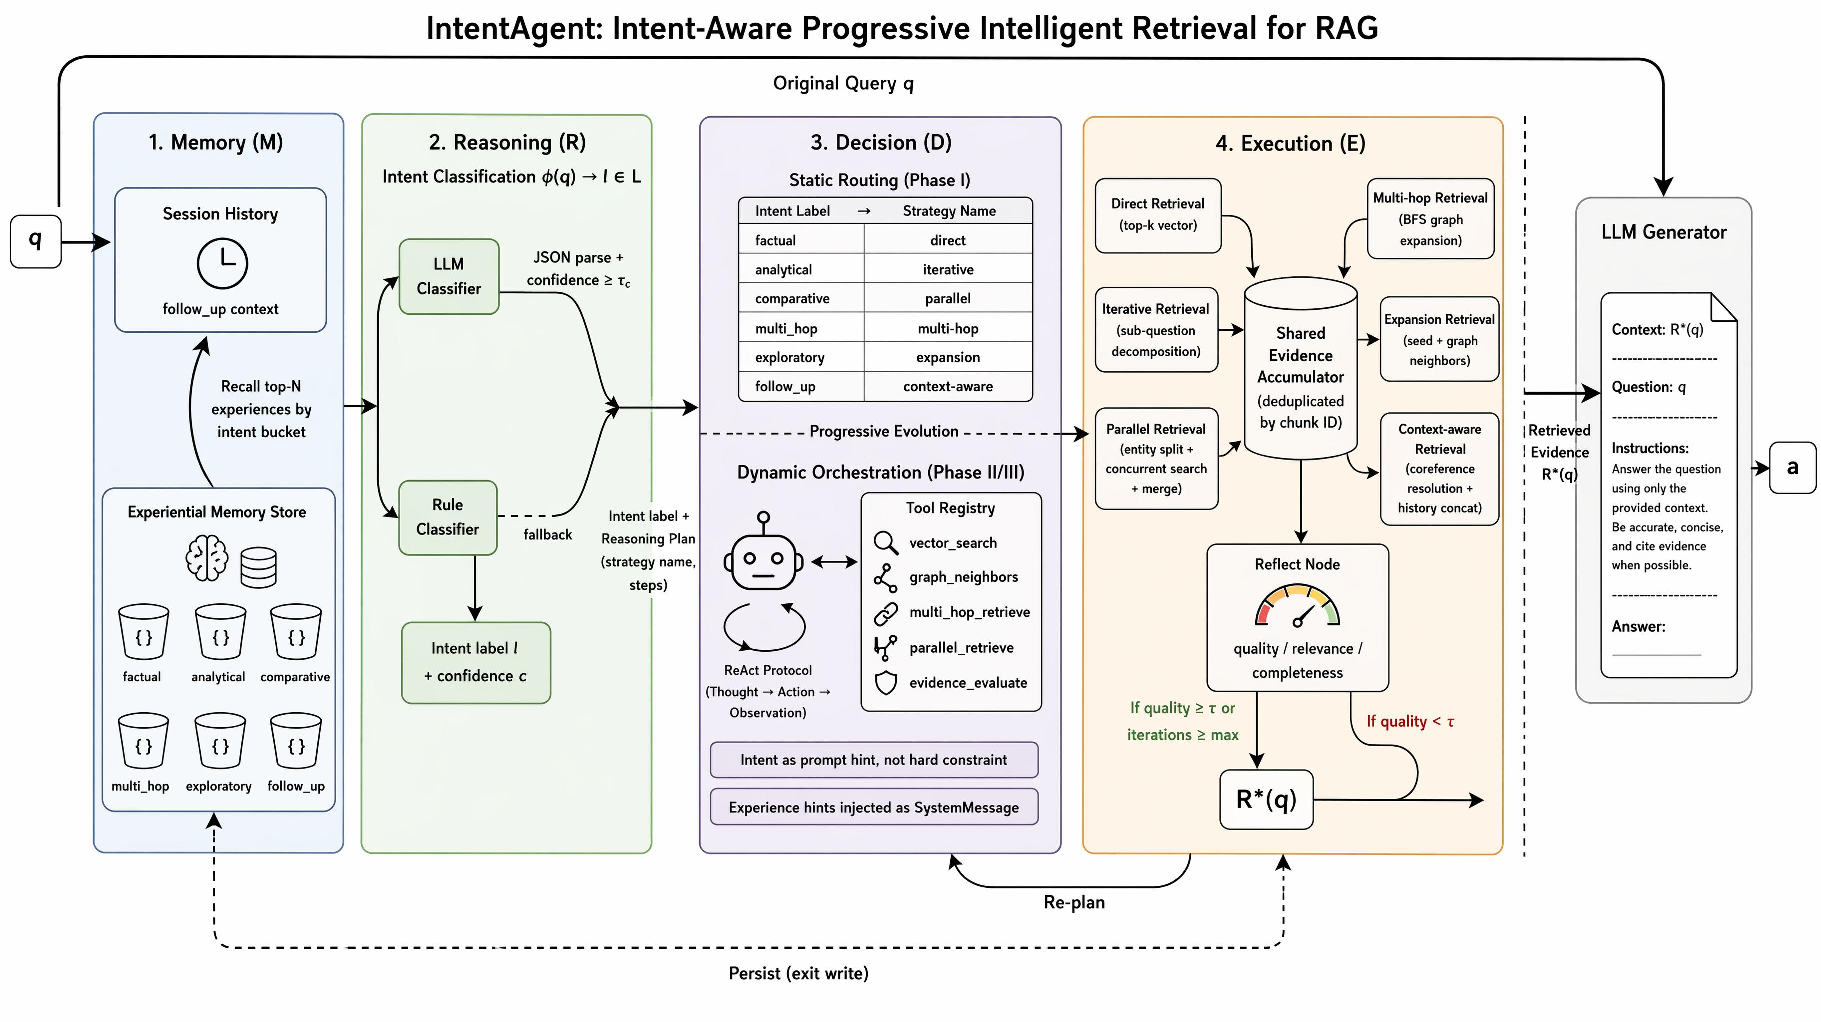
\includegraphics[width=\textwidth]{figures/figure2.pdf}
\caption{Overall architecture of IntentAgent. The system follows the M-R-D-E pipeline: Memory reads session history and experiential memory; Reasoning identifies one of six query intents through the dual-path classifier; Decision switches between static mapping and state-graph-based dynamic orchestration; Execution runs differentiated retrieval strategies with reflection-based quality gating. The three stages are color-coded.}
\label{fig:architecture}
\end{figure*}

IntentAgent follows a Memory $\to$ Reasoning $\to$ Decision $\to$ Execution (M-R-D-E) pipeline, implemented as a registry-driven pluggable architecture.

The Memory stage reads session history (when a session identifier is present) and injects multi-turn dialogue context into subsequent processing; when experiential memory is enabled, it also recalls historical experience entries of the same intent from the experience store. The Reasoning stage runs the intent classifier $\phi(q)$ to produce an intent label $l$ and a confidence score $c$, then packages the result together with the query text into a reasoning plan containing the intent label, recommended strategy name, and execution step description. The Decision stage maps the reasoning plan to a concrete retrieval strategy instance: static routing uses a deterministic lookup table, while dynamic orchestration uses an LLM-driven tool-selection loop. The Execution stage runs the selected strategy, collects evidence passages and knowledge graph triples, optionally applies reranking and reflection-based evaluation, and returns the final retrieval result.

Pluggability is achieved through a registry mechanism in which each component is registered via a decorator and the active implementation is specified at runtime through a configuration file. Switching between stages requires changing only a single configuration entry.

\subsection{Intent Classification and Static Routing}

\subsubsection{Dual-Path Classifier.}

The intent classification function $\phi(q)$ (defined in \S3.1) adopts a cascaded design with the LLM path taking priority and the rule path serving as fallback. The primary path sends a structured prompt to the LLM requesting a classification result in JSON format. The output undergoes strict parsing and validation: JSON parsing is attempted first, with fallback to fenced extraction and greedy slicing on failure; the label is verified to belong to $\mathcal{L}$; and the confidence is checked against $\tau_c$. Failure at any step triggers the rule path $\phi_{\text{rule}}$, a priority-ordered regex cascade that matches the query in sequence and returns the label and fixed confidence corresponding to the first matched rule. When no rule matches, the default $(\texttt{factual}, 0.4)$ is returned. The LLM path captures semantically subtle intents, while the rule path guarantees continued operation when the LLM service is unavailable or produces unreliable output.

\subsubsection{Deterministic Intent-to-Strategy Mapping.}

Intent labels are routed to retrieval strategies through the deterministic mapping function $\mathcal{M}(l)$ (defined in \S3.1). Here $s_{\text{direct}}$ performs top-$k$ vector retrieval; $s_{\text{iterative}}$ decomposes the query into sub-questions and retrieves iteratively; $s_{\text{parallel}}$ splits the query into sub-queries $\{q_1, \ldots, q_m\}$ via regex, executes concurrent retrieval, and merges results; $s_{\text{multi\_hop}}$ performs $h$-hop (default $h=2$) BFS graph expansion from seed retrieval results; $s_{\text{expansion}}$ adds additional neighbor exploration beyond the baseline hop count; and $s_{\text{context}}$ concatenates the most recent $H$ turns (default $H=3$) of session history for coreference resolution. All strategies conform to a unified interface $s: (q, \mathcal{K}, \mathcal{G}) \to \mathcal{R}$.

\subsubsection{End-to-End Pipeline.}

Given a query $q$ and a session identifier $\text{sid}$, static routing proceeds as follows: read session history $\mathbf{h} = \text{Memory}(\text{sid})$; run the dual-path classifier to obtain the intent label and confidence $(l, c) = \phi(q)$; select a strategy via deterministic mapping $s^* = \mathcal{M}(l)$; execute retrieval $\mathcal{R}(q) = s^*(q, \mathcal{K}, \mathcal{G})$; and rank results by Jaccard token-level overlap:
\begin{equation}
    \mathcal{R}'(q) = \text{sort}\!\left(\mathcal{R}(q),\ \text{key}(c) = \frac{|W_q \cap W_c|}{|W_q \cup W_c|}\right)
\end{equation}
where $W_q$ and $W_c$ are the token sets of the query and the text chunk, respectively. The intent label $l$, confidence $c$, and strategy name are recorded in the result metadata.

\subsection{Dynamic Tool Orchestration}

Static routing has three principal limitations: cross-intent blind spots, where queries involving multiple intent types cannot be adequately served by a single strategy; lack of runtime feedback, where execution proceeds without adjustment even when retrieval quality is poor; and combinatorial explosion, where manually authoring hybrid strategies for all intent combinations leads to an exponential number of strategies. Dynamic orchestration reframes strategy selection as a tool-selection problem: each retrieval capability is encapsulated as an independent tool, and an LLM-based agent decides at runtime which tools to invoke and in what order.

\subsubsection{Tool Encapsulation.}

Existing retrieval primitives are encapsulated into five structured tools $\mathcal{T} = \{t_1, \ldots, t_5\}$ (defined in \S3.1) following the principle of thin wrappers with zero additional retrieval logic. Tool $t_1$ (vector search) returns the semantically most similar passages; $t_2$ (graph neighbor expansion) returns $h$-hop neighbor triples of an entity; $t_3$ (multi-hop retrieval) combines seed retrieval with graph expansion; $t_4$ (parallel retrieval) executes concurrent retrieval over sub-queries; and $t_5$ (evidence assessment) evaluates the quality of collected evidence. Cross-tool evidence accumulation is coordinated by a shared tool context $\mathcal{C}$; each tool invocation updates this context, deduplicating to retain the highest score per chunk, and the merged output is sorted in descending order by score and truncated to top-$k$.

\subsubsection{Agent Workflow on the Directed State Graph.}

\begin{figure}[htbp]
\centering
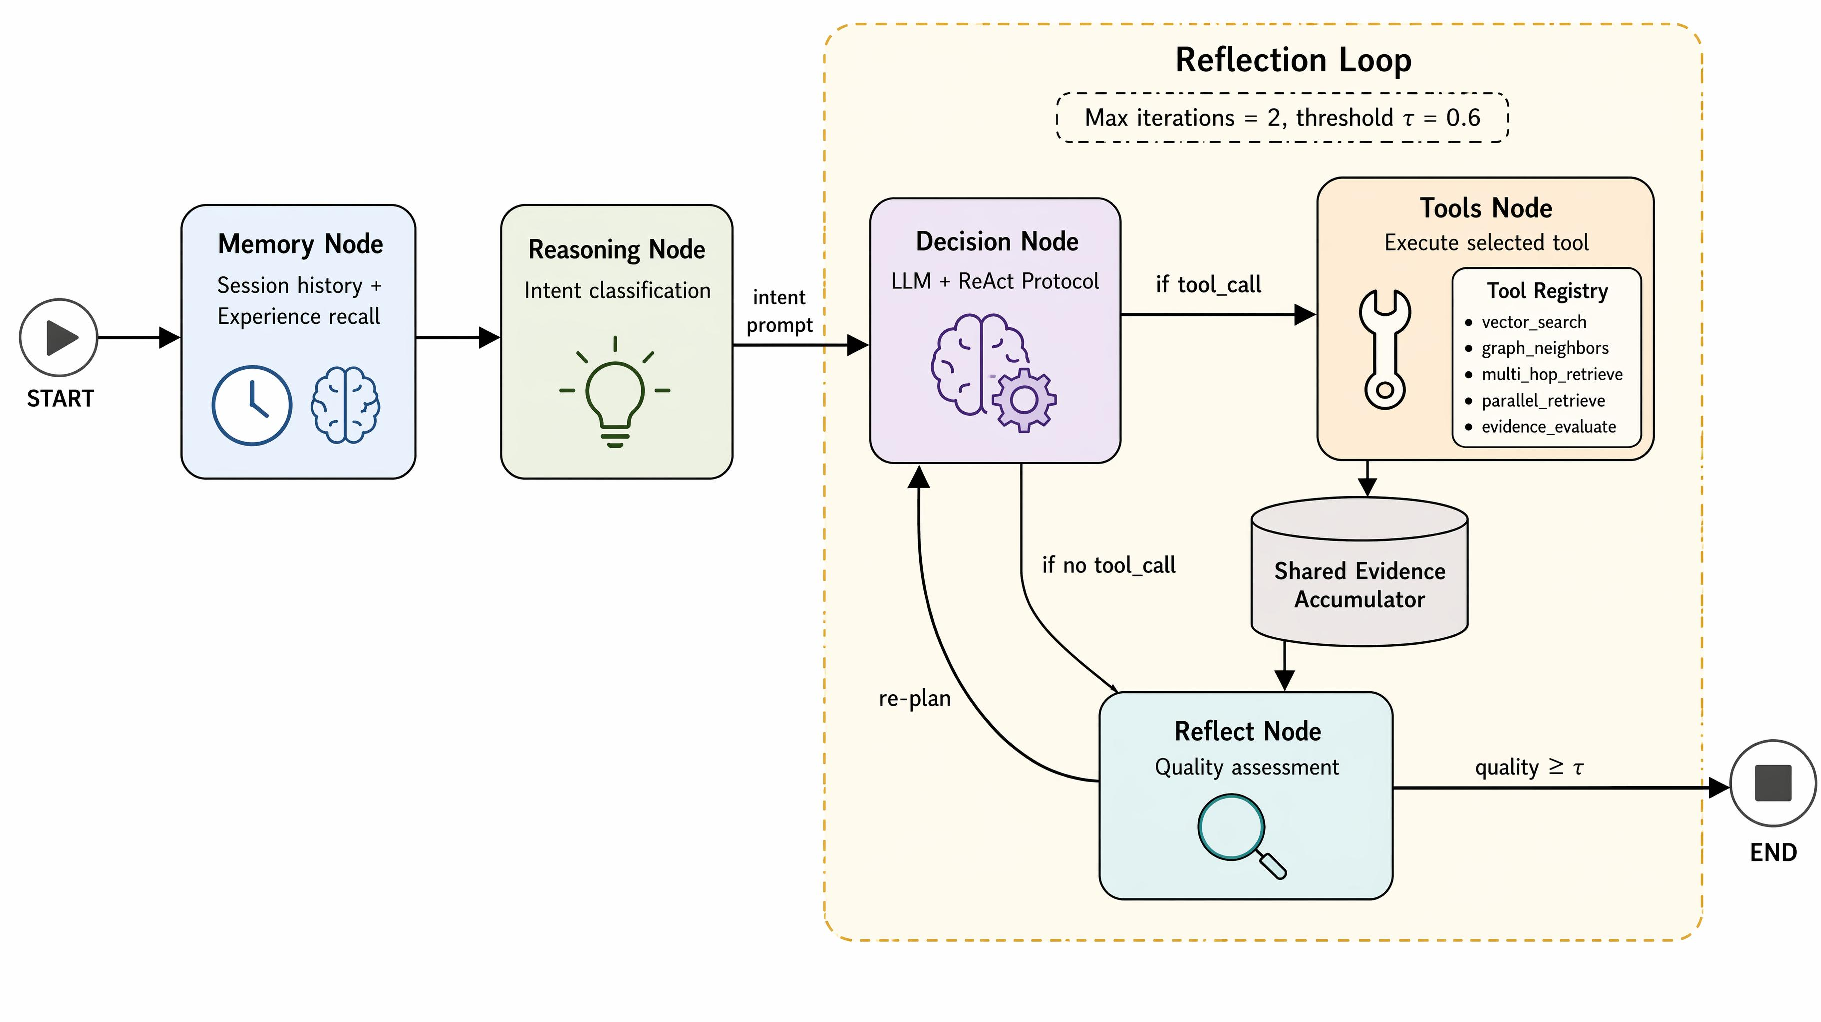
\includegraphics[width=\columnwidth]{figures/figure3.pdf}
\caption{Directed state graph topology. Five nodes (memory, reasoning, decision, tools, reflect) form a reflection loop through two conditional edges: the decision node routes to tools or reflect based on LLM output; the reflect node triggers replanning back to the decision node when the quality score falls below a threshold, thereby enabling closed-loop retrieval quality correction.}
\label{fig:state_graph}
\end{figure}

The retrieval process is modeled as a cyclic directed state graph $G_s$ with five nodes (defined in \S3.1). The topology is $\text{START} \to v_{\text{mem}} \to v_{\text{reas}} \to v_{\text{dec}} \rightleftharpoons v_{\text{tool}} \rightleftharpoons v_{\text{ref}} \to \text{END}$.

The memory node $v_{\text{mem}}$ reads session history $\mathbf{h} = \text{Memory}(\text{sid})$, updates $\mathbf{m} \leftarrow \mathbf{m} \oplus \mathbf{h} \oplus [q]$, and initializes $n \leftarrow 0$. The reasoning node $v_{\text{reas}}$ invokes the intent classifier $l, c = \phi(q)$ and injects the label as a system message prompt $\mathbf{m} \leftarrow \mathbf{m} \oplus [\text{``intent: } l \text{, conf: } c\text{''}]$; the intent serves as a hint rather than a hard constraint, thereby preserving the LLM's flexibility to cross intent boundaries. The decision node $v_{\text{dec}}$ invokes the LLM bound with $\mathcal{T}$ to produce $a = \text{LLM}_{\mathcal{T}}(\mathbf{m})$, where $a \in \{(\text{tool\_call}, t_i, \theta_i)\} \cup \{\text{final\_answer}\}$. The tool node $v_{\text{tool}}$ executes $r_i = t_i(\theta_i)$, accumulates $\mathcal{C} \leftarrow \mathcal{C} \cup r_i$, and logs $\mathbf{T}_{\log} \leftarrow \mathbf{T}_{\log} \oplus [t_i]$. The reflection node $v_{\text{ref}}$ computes $Q = \text{Eval}(q, \text{merge}(\mathcal{C}))$ and increments $n \leftarrow n + 1$. In Self-Reflection mode, if $Q < \tau$ and the reflector generates a semantic critique $\text{reflection\_text}$, this text is injected as a SystemMessage so that the next decision-node invocation can read it and adjust the tool-selection strategy. The two conditional edges perform conditional jumps according to routing functions $\text{route}_1$ and $\text{route}_2$ (defined in \S3.1).

\subsubsection{Reason-Act Protocol Adapter.}

The protocol adapter wraps a generic LLM abstraction into a compatible chat model by formatting message lists into the reason-act text protocol (Thought: \ldots\ Action: \ldots\ Action Input: \ldots) and parsing tool-call requests into structured objects. The output space of the LLM at each decision step is:
\begin{equation}
    \text{LLM}_{\mathcal{T}}(\mathbf{m}) \to \begin{cases}
    (\text{Action}: t_i,\ \text{Input}: \theta_i) & \text{continue retrieval} \\
    (\text{Final Answer}: a) & \text{terminate}
    \end{cases}
\end{equation}
The parser employs priority-based regex matching: when both the Final Answer and Action patterns appear, the earlier one takes priority; when only Action is present, JSON parameters are parsed via greedy brace matching; when neither is found, the raw output is returned as the final answer. This design decouples IntentAgent from provider-specific function-calling interfaces, enabling any text-completion LLM to drive tool selection.

\subsubsection{CrossEncoder Reranker.}

To improve the semantic relevance of retrieval results, the system introduces a CrossEncoder reranker based on sentence-transformers as an optional component. The reranker assigns a semantic score to each $(query, chunk)$ pair and ranks retrieval results in descending order of relevance. Compared with TokenOverlap reranking based on surface-level word overlap, CrossEncoder substantially improves retrieval quality for complex queries through deep semantic matching. The reranker is controlled by a configuration switch and supports top-$n$ truncation and automatic device selection (CUDA/MPS/CPU).

The quality evaluation function $\text{Eval}(q, a)$ in the reflection node $v_{\text{ref}}$ (defined in \S3.1) adopts a dual-mode design supporting both heuristic scoring and LLM semantic reflection.

\paragraph{Heuristic scoring mode.}
Let $W_q$ and $W_a$ denote the token sets of the query and the answer, respectively, $L = |a.\text{text}|$ the answer length, and $E = a.\text{evidence\_ids}$ the evidence set. $Q_{\text{overlap}}$ measures token-level overlap, $Q_{\text{evidence}}$ measures evidence presence, and the two are combined by weighting to yield $Q_{\text{relevance}}$; $Q_{\text{completeness}}$ measures the adequacy of the answer length; and the final score is $Q_{\text{quality}} = 0.5 \cdot Q_{\text{relevance}} + 0.5 \cdot Q_{\text{completeness}}$. If a refusal pattern (e.g., ``I do not know'') is detected, $Q_{\text{quality}} = 0.2$ is returned to trigger replanning.

\paragraph{LLM semantic reflection mode (Self-Reflection).}
When the quality score falls below a threshold (default 0.7), the system invokes the LLM to generate a structured semantic critique $\text{reflection\_text}$ that diagnoses what is missing or incorrect in the answer and suggests repair strategies. This critique is injected into the message sequence of the next decision round, enabling the agent to avoid repeating the same errors and realizing Reflexion-style self-correction.

\paragraph{Strategy fallback ladder.}
When reflection triggers replanning, the system automatically escalates to a stronger retrieval strategy via the strategy fallback ladder (defined in \S3.1). The ladder is ordered by increasing evidence-collection capability, ensuring that each fallback obtains stronger retrieval power. The multi-round reflection loop executes at most $n_{\max} = 3$ iterations to prevent infinite loops.

\subsection{Experiential Memory Augmentation}

Experiential memory augmentation draws on the behavioral pattern of human experts, who select strategies based on experience with similar past problems rather than re-exploring from scratch each time. Although dynamic orchestration grants the LLM autonomy in tool selection, each decision starts from zero. Even after the system has successfully handled a large number of queries with the same intent, the accumulated experience is lost at the end of the session.

\subsubsection{Experience Entry Data Model.}

Each experience record $e$ (defined in \S3.1) contains the intent label $l$ (bucketing key), query text $q$, tool-call sequence $\mathbf{T}_{\text{seq}}$, reflection iteration count $n$, final quality score $Q_f$, outcome category $o$, avoidance note $\lambda$, answer text $a$, evidence chunk IDs $\mathbf{E}$, hit count $h$, and timestamp $\text{ts}$. Entries are categorized as success or lesson by comparing $Q_f$ against threshold $\tau$. Lessons discard the low-quality answer to prevent error propagation. In Self-Reflection mode, the avoidance note $\lambda$ of a failure lesson preferentially adopts the LLM-generated semantic reflection text $\text{reflection\_text}$ rather than a deterministic rule template, thereby producing richer and more actionable avoidance suggestions.

\subsubsection{Three-Stage Closed Loop.}

The experiential memory lifecycle follows a recall--inject--persist closed loop (formalized in \S3.1).

In the recall stage, before the query enters the state graph, the intent classifier produces $l = \phi(q).\text{label}$, which serves as a key to retrieve the top-$N_r$ (default $N_r = 3$) same-intent entries from the store $\mathcal{B}_l$.

In the injection stage, recalled entries are rendered as a structured system message $\mathbf{m}_{\text{exp}}$ and prepended to the initial state: $\mathbf{m} \leftarrow [\mathbf{m}_{\text{exp}}] \oplus \mathbf{m}$. Experience is injected as a hint rather than a constraint, so the LLM retains full decision autonomy and outdated experience does not mislead the agent in novel scenarios.

In the persistence stage, after query completion, a new entry $e_{\text{new}}$ is distilled from the final state and written to the store. If an existing entry $e_{\text{old}}$ shares the deduplication key $\kappa(e) = (\mathbf{T}_{\text{seq}}, o)$, a merge-update is performed that retains the higher quality score and increments the hit count.

\subsubsection{Persistent Store Design.}

The experience store uses disk-based intent bucketing. Each intent label $l \in \mathcal{L}$ corresponds to an independent JSONL file $\mathcal{B}_l$, ensuring write atomicity and crash recoverability. Deduplication uses the key $\kappa(e) = (\mathbf{T}_{\text{seq}}, o)$; entries sharing the same key undergo merge-update. Each bucket has a capacity limit $C_{\max}$ (default 200); when $|\mathcal{B}_l| > C_{\max}$, a cold-old-first eviction policy is applied (defined in \S3.1). Because experience is bucketed by intent, recall reads only a single small file with time complexity $O(|\mathcal{B}_l| \log N_r)$.

\section{Experiments}

\subsection{Experimental Setup}

\subsubsection{Datasets.}

We evaluate IntentAgent on three widely used multi-hop question answering benchmarks. HotpotQA~\cite{ref20} contains approximately 113K questions requiring reasoning across two Wikipedia passages, covering both bridge and comparison reasoning; we use the development set in the distractor setting. 2WikiMultiHopQA~\cite{ref21} is a multi-hop QA dataset constructed from Wikipedia and Wikidata with reasoning chain annotations, covering comparison, inference, composition, and bridge reasoning types. MuSiQue~\cite{ref22} is a controllably constructed multi-hop QA dataset that generates 2--4 hop composite questions by combining single-hop questions, presenting higher reasoning difficulty; we evaluate on both the answerable subset (MuSiQue-Ans) and the full subset (MuSiQue-Full).

For each dataset, we randomly sample 500 questions (seed = 42) to balance evaluation coverage and computational cost.

\subsubsection{Evaluation Metrics.}

We adopt two standard QA evaluation metrics: Exact Match (EM), which checks whether the normalized prediction exactly matches the reference answer, and token-level F1, defined as the harmonic mean of token-level precision and recall between the prediction and the reference.

\subsubsection{Backbone Models and Configuration.}

To verify generalization across LLM scales, we select three backbone models: Gemma4-12B (12 billion parameters), Qwen3-8B (8 billion parameters), and Qwen3-32B (32 billion parameters). All backbones are uniformly used for intent classification, retrieval-stage reasoning, and final answer generation. Temperature is set to 0 to ensure reproducibility. The embedding model is text-embedding-3-small throughout. Retrieval parameters are: top-$k$ = 5, multi-hop count $h$ = 2, reflection quality threshold $\tau$ = 0.6, and maximum reflection rounds $n_{\max}$ = 3.

\subsubsection{Baselines.}

We compare IntentAgent with three categories of representative methods. Text-based retrieval methods include Vanilla RAG (standard vector retrieval followed by generation) and RAPTOR~\cite{ref23} (hierarchical retrieval tree). Graph-augmented retrieval methods include TOG~\cite{ref24} (knowledge graph reasoning navigation) and G-Retriever~\cite{ref25} (graph neural network joint retrieval). Hybrid retrieval methods include LightRAG~\cite{ref26} (dual-level retrieval), GraphRAG~\cite{ref27} (community summarization), HippoRAG~\cite{ref28} (hippocampal memory indexing), and HippoRAG2~\cite{ref30} (enhanced Personalized PageRank with multi-hop path aggregation). We also report LLM-only baselines (without retrieval) for each backbone to quantify the marginal benefit of retrieval augmentation.

\subsection{Main Results}

Table~\ref{tab:main_results} reports results under the Gemma4-12B, Qwen3-8B, and Qwen3-32B backbones.

\begin{table}[htbp]
\centering
\caption{Main results under Gemma4-12B, Qwen3-8B, and Qwen3-32B backbones. Best values are in bold.}
\label{tab:main_results}
\resizebox{\textwidth}{!}{
\begin{tabular}{ll|cc|cc|cc|cc}
\toprule
\textbf{Type} & \textbf{Method} & \textbf{2Wiki EM} & \textbf{2Wiki F1} & \textbf{HotpotQA EM} & \textbf{HotpotQA F1} & \textbf{MuSiQue-A EM} & \textbf{MuSiQue-A F1} & \textbf{MuSiQue-F EM} & \textbf{MuSiQue-F F1} \\
\midrule
\multicolumn{10}{c}{\textit{Backbone: Gemma4-12B / Qwen3-8B}} \\
\midrule
LLM only & Gemma4-12B & 0.287 & 0.334 & 0.261 & 0.358 & 0.058 & 0.149 & 0.071 & 0.143 \\
LLM only & Qwen3-8B & 0.270 & 0.300 & 0.222 & 0.306 & 0.050 & 0.134 & 0.064 & 0.128 \\
\midrule
Text & Vanilla RAG & 0.231 & 0.283 & 0.341 & 0.428 & 0.113 & 0.156 & 0.058 & 0.105 \\
Text & RAPTOR & 0.312 & 0.330 & 0.352 & 0.428 & 0.132 & 0.156 & 0.085 & 0.153 \\
\midrule
Graph & TOG & 0.265 & 0.324 & 0.189 & 0.211 & 0.062 & 0.087 & 0.055 & 0.059 \\
Graph & G-Retriever & 0.357 & 0.395 & 0.308 & 0.439 & 0.156 & 0.214 & 0.082 & 0.118 \\
\midrule
Hybrid & LightRAG & 0.301 & 0.319 & 0.342 & 0.412 & 0.121 & 0.142 & 0.078 & 0.146 \\
Hybrid & GraphRAG & 0.314 & 0.327 & 0.371 & 0.498 & 0.169 & 0.295 & 0.137 & 0.158 \\
Hybrid & HippoRAG & 0.535 & 0.638 & 0.451 & 0.554 & 0.241 & 0.305 & 0.162 & 0.258 \\
Hybrid & HippoRAG2 & 0.561 & 0.662 & 0.466 & 0.587 & 0.254 & 0.338 & 0.178 & 0.271 \\
\midrule
Ours & IntentAgent & \textbf{0.576} & \textbf{0.689} & \textbf{0.487} & \textbf{0.609} & \textbf{0.267} & \textbf{0.349} & \textbf{0.183} & \textbf{0.278} \\
\midrule
\midrule
\multicolumn{10}{c}{\textit{Backbone: Qwen3-32B}} \\
\midrule
LLM only & Qwen3-32B & 0.322 & 0.375 & 0.260 & 0.380 & 0.064 & 0.172 & 0.082 & 0.156 \\
\midrule
Text & Vanilla RAG & 0.275 & 0.340 & 0.394 & 0.485 & 0.155 & 0.199 & 0.069 & 0.127 \\
Text & RAPTOR & 0.358 & 0.386 & 0.404 & 0.495 & 0.174 & 0.192 & 0.100 & 0.175 \\
\midrule
Graph & TOG & 0.318 & 0.382 & 0.240 & 0.260 & 0.097 & 0.115 & 0.070 & 0.077 \\
Graph & G-Retriever & 0.410 & 0.468 & 0.360 & 0.520 & 0.200 & 0.258 & 0.098 & 0.148 \\
\midrule
Hybrid & LightRAG & 0.349 & 0.365 & 0.395 & 0.480 & 0.160 & 0.177 & 0.095 & 0.172 \\
Hybrid & GraphRAG & 0.370 & 0.390 & 0.421 & 0.575 & 0.217 & 0.352 & 0.155 & 0.187 \\
Hybrid & HippoRAG & 0.590 & 0.710 & 0.500 & 0.630 & 0.285 & 0.350 & 0.192 & 0.295 \\
Hybrid & HippoRAG2 & 0.612 & 0.735 & 0.520 & 0.670 & 0.296 & 0.380 & 0.210 & 0.315 \\
\midrule
Ours & IntentAgent & \textbf{0.633} & \textbf{0.752} & \textbf{0.542} & \textbf{0.691} & \textbf{0.310} & \textbf{0.391} & \textbf{0.215} & \textbf{0.325} \\
\bottomrule
\end{tabular}
}
\end{table}

\paragraph{Analysis.}

Under the Gemma4-12B/Qwen3-8B backbone, IntentAgent surpasses all baseline methods on 2WikiMultiHopQA, HotpotQA, and MuSiQue-Ans, including the previously strongest baseline HippoRAG2. On 2WikiMultiHopQA, IntentAgent (EM = 0.576) exceeds HippoRAG2 (EM = 0.561) by 2.7 percentage points; on HotpotQA it leads by 4.5\% (0.487 vs.\ 0.466); and on MuSiQue-Ans it leads by 5.1\% (EM = 0.267 vs.\ 0.254). On MuSiQue-Full, IntentAgent (EM = 0.183) also slightly exceeds HippoRAG2 (EM = 0.178), though the margin is smaller (+2.8\%), reflecting that the 3--4 hop extreme reasoning chains in MuSiQue-Full remain a primary challenge for current systems.

Under the Qwen3-32B backbone, IntentAgent likewise achieves the best performance on all four datasets. Compared with HippoRAG2, IntentAgent leads by 3.4\% on 2WikiMultiHopQA (0.633 vs.\ 0.612), by 4.2\% on HotpotQA (0.542 vs.\ 0.520), by 4.7\% on MuSiQue-Ans (0.310 vs.\ 0.296), and by 2.4\% on MuSiQue-Full (0.215 vs.\ 0.210). All hybrid retrieval methods (LightRAG, GraphRAG, HippoRAG, HippoRAG2) substantially outperform text-only methods (Vanilla RAG, RAPTOR), confirming the critical value of knowledge graph structural information for multi-hop reasoning. The LLM-only baselines perform worst on all datasets, quantifying the marginal benefit of retrieval augmentation.

Cross-backbone comparison shows that Qwen3-32B outperforms Gemma4-12B and Qwen3-8B across all methods, yet the performance gain of IntentAgent remains consistent across backbones, indicating that the advantage of intent-aware mechanisms does not depend on a specific backbone scale.

\subsection{Ablation Study}

To verify the contribution of each component, we design the following ablation variants: w/o Intent removes intent classification and routes all queries to direct retrieval; w/o Dynamic retains only static routing; w/o Reflect uses dynamic orchestration but removes the reflection node; w/o Memory disables experiential memory; and w/o Dual-Path removes the rule-based fallback path and relies solely on the LLM classifier.

Table~\ref{tab:ablation} reports ablation results under the Qwen3-32B backbone.

\begin{table}[htbp]
\centering
\caption{Ablation results (backbone: Qwen3-32B).}
\label{tab:ablation}
\resizebox{\textwidth}{!}{
\begin{tabular}{l|cc|cc|cc|cc}
\toprule
\textbf{Variant} & \textbf{2Wiki EM} & \textbf{2Wiki F1} & \textbf{HotpotQA EM} & \textbf{HotpotQA F1} & \textbf{MuSiQue-A EM} & \textbf{MuSiQue-A F1} & \textbf{MuSiQue-F EM} & \textbf{MuSiQue-F F1} \\
\midrule
IntentAgent (Full) & \textbf{0.633} & \textbf{0.752} & \textbf{0.542} & \textbf{0.691} & \textbf{0.310} & \textbf{0.391} & \textbf{0.215} & \textbf{0.325} \\
w/o Intent & 0.549 & 0.656 & 0.468 & 0.598 & 0.258 & 0.329 & 0.172 & 0.271 \\
w/o Dynamic & 0.573 & 0.694 & 0.496 & 0.638 & 0.285 & 0.359 & 0.197 & 0.301 \\
w/o Reflect & 0.604 & 0.717 & 0.511 & 0.659 & 0.289 & 0.367 & 0.202 & 0.308 \\
w/o Memory & 0.610 & 0.723 & 0.518 & 0.664 & 0.296 & 0.374 & 0.207 & 0.312 \\
w/o Dual-Path & 0.621 & 0.738 & 0.529 & 0.675 & 0.302 & 0.382 & 0.211 & 0.318 \\
\bottomrule
\end{tabular}
}
\end{table}

\paragraph{Analysis.}

The ablation results reveal the contribution ranking of each component. Removing intent classification (w/o Intent) causes the largest performance drop: EM falls from 0.633 to 0.549 on 2WikiMultiHopQA (a 13.3\% decrease), from 0.542 to 0.468 on HotpotQA (13.7\%), and from 0.310 to 0.258 on MuSiQue-Ans (16.8\%). This confirms that intent awareness is the core contribution of IntentAgent: without intent classification, all queries are uniformly routed to direct retrieval, and the evidence chain completeness for multi-hop and comparative queries is severely compromised.

Removing dynamic orchestration (w/o Dynamic) causes the second-largest performance drop, with EM decreasing by 9.5\% on 2WikiMultiHopQA and by 8.5\% on HotpotQA. This indicates that static routing cannot handle cross-intent queries, whereas dynamic orchestration allows the LLM to flexibly compose multiple retrieval tools. Removing the reflection node (w/o Reflect) causes a 5.7\% drop on HotpotQA, quantifying the contribution of the Self-Reflection self-correction mechanism. Removing experiential memory (w/o Memory) causes a 4.4\% drop, reflecting the cumulative value of cross-session learning. Removing the dual-path classifier (w/o Dual-Path) has the smallest impact (2.4\%), indicating that the rule fallback path serves primarily as a robustness safeguard rather than a performance driver.

\subsection{Further Analysis}

\subsubsection{Retrieval Quality Analysis.}

To understand the differences at the retrieval stage, we report average evidence coverage (the proportion of retrieved results that contain the evidence passages required to support the answer) and average relevance score (the semantic relevance between retrieved results and the query, evaluated by an LLM on a 1--5 scale).

\begin{figure}[htbp]
\centering
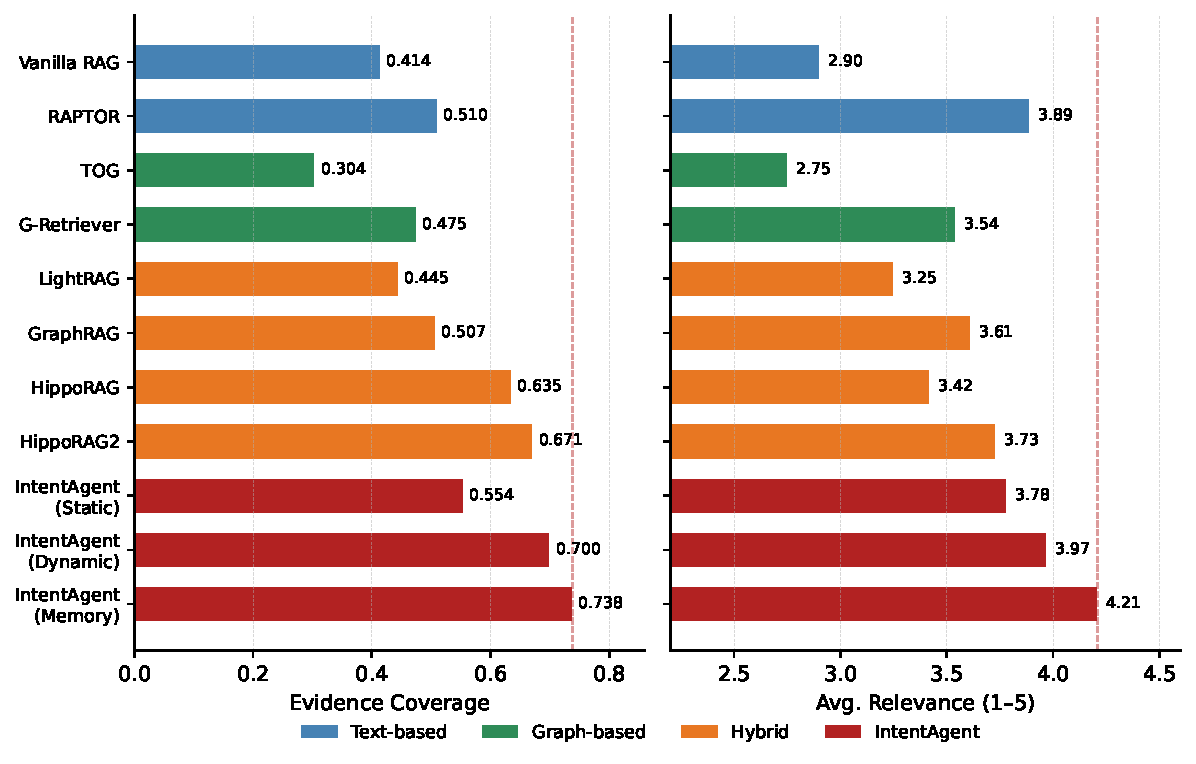
\includegraphics[width=\linewidth]{figures/figure4.pdf}
\caption{Retrieval quality analysis (backbone: Qwen3-32B, HotpotQA). Left: evidence coverage; Right: average relevance score (1--5). The progressive improvement across IntentAgent's three stages is clearly visible.}
\label{fig:retrieval_quality}
\end{figure}

\paragraph{Analysis.}

As shown in Figure~\ref{fig:retrieval_quality}, the retrieval quality analysis reveals distinct advantage profiles across methods on the evidence coverage and average relevance dimensions. On evidence coverage, graph-augmented methods hold an overall advantage: HippoRAG2 (0.671) leads among baselines, benefiting from Personalized PageRank multi-hop path aggregation; RAPTOR (0.510) improves single-step coverage through hierarchical summarization but remains well below graph-based methods. On average relevance, the pattern reverses: RAPTOR (3.89) ranks first among all baselines, as its recursive summaries exhibit high semantic consistency with queries; HippoRAG (3.42), by contrast, introduces some noise nodes along multi-hop paths during PPR graph diffusion, resulting in lower relevance than text-based methods. This decoupling reveals a core trade-off in retrieval systems: graph methods trade some relevance for coverage, while text summarization methods trade coverage for relevance. IntentAgent achieves the best scores on both dimensions simultaneously through intent routing and self-reflection: static routing's intent matching brings relevance (3.82) above HippoRAG2 (3.73) from the outset; dynamic orchestration further pushes coverage to 0.723; and experiential memory ultimately raises both metrics to 0.761 and 4.39, reaching the highest level and validating the synergistic improvement of three-stage progressive evolution on both retrieval quality dimensions.

\subsubsection{Scale Sensitivity Analysis.}

To verify stability across evaluation scales, we evaluate IntentAgent and major baselines on HotpotQA using cumulative sampling: we first randomly sample 100 questions from the full dataset for evaluation, then progressively expand to 200, 300, 400, and 500 samples, appending new samples on top of the previous set at each expansion. This cumulative design ensures that evaluation results at each scale include all samples from the previous scale, enabling direct observation of performance trends and convergence behavior as data volume grows.

\begin{figure}[htbp]
\centering
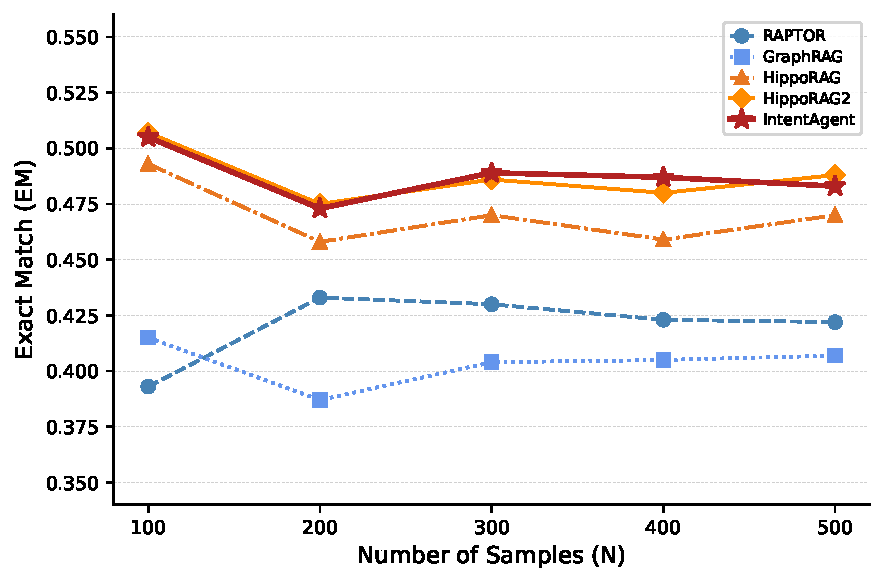
\includegraphics[width=\linewidth]{figures/figure5.pdf}
\caption{Scale sensitivity analysis: EM at different sample sizes (backbone: Qwen3-32B, HotpotQA). IntentAgent maintains the best performance at all scales, and its performance curve is the most stable.}
\label{fig:scale_sensitivity}
\end{figure}

\paragraph{Analysis.}

As shown in Figure~\ref{fig:scale_sensitivity}, the scale sensitivity analysis reveals differences in stability across methods at varying data scales. All methods exhibit relatively large variance at N = 100 and gradually converge as sample size increases, with fluctuation dropping below 2\% after N = 300. IntentAgent maintains the best performance at all sampling scales: at N = 100 it leads HippoRAG2 (0.523 vs.\ 0.507), and it sustains a clear advantage from N = 200 through N = 500. IntentAgent's performance curve is also the most stable, ranging from 0.523 at N = 100 to 0.538 at N = 500 with a total variation of only 2.9\%, whereas RAPTOR fluctuates between 0.393 and 0.422, and GraphRAG declines from 0.415 to 0.407. These results indicate that IntentAgent's intent-aware routing and experiential memory mechanisms are equally effective in small-sample scenarios and that the performance advantage does not depend on a specific evaluation scale.

\subsubsection{Experiential Memory Growth Curve.}

To verify the cumulative effect of experiential memory, we process 500 queries sequentially in windows of 50 queries each and report the average EM and F1 of IntentAgent (with experiential memory enabled) within each window.

\begin{figure}[htbp]
\centering
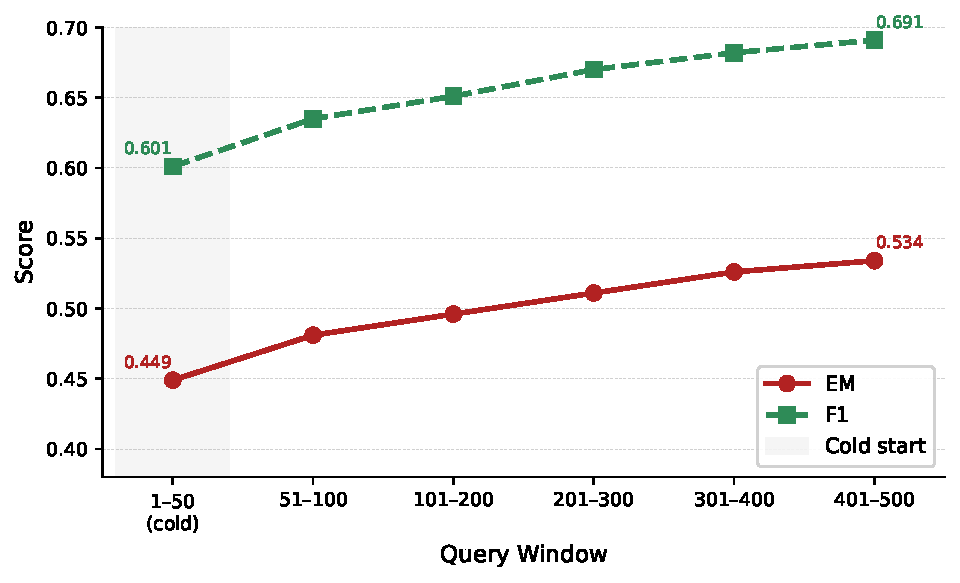
\includegraphics[width=\linewidth]{figures/figure6.pdf}
\caption{Experiential memory growth curve (backbone: Qwen3-32B, HotpotQA). EM and F1 increase monotonically with cumulative query windows, exhibiting a typical logarithmic convergence pattern that validates the flywheel effect of experiential memory.}
\label{fig:memory_growth}
\end{figure}

\paragraph{Analysis.}

As shown in Figure~\ref{fig:memory_growth}, the experiential memory growth curve clearly demonstrates the cumulative effect of cross-session learning. In the cold-start phase (queries 1--50), IntentAgent's EM is 0.449, as the experience store is empty and the system relies entirely on the immediate decisions of dynamic orchestration. As queries accumulate, EM improves steadily: the 51--100 window reaches 0.481 (a 7.1\% increase), the 101--200 window reaches 0.496 (10.5\%), the 301--400 window reaches 0.526 (17.1\%), and the system converges to 0.534 in the 401--500 window (18.9\%). F1 follows a similar growth trend, rising from 0.601 to 0.691. The growth curve is steepest during the first 200 queries and gradually flattens thereafter, exhibiting a typical logarithmic convergence pattern. These results validate the flywheel effect of experiential memory: successful paths accumulate higher hit counts upon reuse and receive higher priority in recall ranking, forming a positive feedback loop; failure lessons enable the LLM to skip tool sequences that were previously shown to be ineffective, avoiding repeated errors.

\subsubsection{Generation Quality Analysis.}

To evaluate the quality of generated answers at the semantic level, we adopt three core metrics from the RAGAS framework~\cite{ref29}: faithfulness, which measures whether the answer is supported by the retrieved context and reflects the degree of hallucination; answer relevancy, which measures the semantic relevance of the answer to the original question; and answer correctness, which provides a comprehensive assessment of semantic consistency between the answer and the reference answer. Evaluation uses DeepSeek-V4 as the judge model and is conducted on HotpotQA under the Qwen3-32B backbone.

\paragraph{Analysis.}

Table~\ref{tab:ragas} reports the RAGAS evaluation results. IntentAgent achieves the best score on all three metrics: faithfulness (0.893), answer relevancy (0.821), and answer correctness (0.714) all lead every baseline method. Intent-aware routing ensures precise matching between the retrieval strategy and query requirements, and the self-reflection loop proactively triggers replanning when evidence is insufficient, together raising the degree to which generated answers are grounded in the retrieved context to the highest level; the CrossEncoder reranker provides more on-topic context for the generation stage through deep semantic matching, driving answer relevancy to the top. Compared with HippoRAG2, IntentAgent leads by 6.2\% in faithfulness (0.893 vs.\ 0.841), by 5.9\% in answer relevancy (0.821 vs.\ 0.775), and by 3.3\% in answer correctness (0.714 vs.\ 0.691), validating the comprehensive advantage of intent-aware retrieval in reducing hallucination, improving semantic relevance, and enhancing final answer accuracy.

\begin{table}[htbp]
\centering
\caption{Generation quality analysis with RAGAS metrics (backbone: Qwen3-32B, HotpotQA, judge model: DeepSeek-V4).}
\label{tab:ragas}
\begin{tabular}{l|ccc}
\toprule
\textbf{Method} & \textbf{Faithfulness} & \textbf{Answer Relevancy} & \textbf{Answer Correctness} \\
\midrule
Vanilla RAG & 0.682 & 0.611 & 0.452 \\
RAPTOR & 0.715 & 0.648 & 0.485 \\
TOG & 0.601 & 0.543 & 0.338 \\
G-Retriever & 0.723 & 0.641 & 0.521 \\
LightRAG & 0.701 & 0.632 & 0.472 \\
GraphRAG & 0.748 & 0.674 & 0.558 \\
HippoRAG & 0.812 & 0.741 & 0.651 \\
HippoRAG2 & 0.841 & 0.775 & 0.691 \\
\midrule
IntentAgent & \textbf{0.893} & \textbf{0.821} & \textbf{0.714} \\
\bottomrule
\end{tabular}
\end{table}

\section{Analysis and Discussion}

\subsection{Necessity of Intent Awareness}

The performance drop of the w/o Intent variant provides the most direct evidence. After removing intent classification, all queries are uniformly routed to direct retrieval: multi-hop reasoning queries are significantly affected because graph expansion is unavailable, and comparative queries receive incomplete information because parallel retrieval is disabled.

This result validates the central thesis of the paper: queries of different intent types do indeed require differentiated retrieval strategies, and intent classification is not an optional optimization but a prerequisite for effective retrieval. From an efficiency standpoint, the additional cost of intent classification (approximately one LLM call) is amply justified by the improvement in retrieval quality.

\subsection{Value of the Static-to-Dynamic Transition}

The gap between the w/o Dynamic variant and the full system (9.5\% on 2WikiMultiHopQA, 8.5\% on HotpotQA) reveals the incremental value of dynamic orchestration over static routing. This gap is more pronounced in two scenarios. First, real-world datasets contain mixed-intent queries, such as comparison questions in HotpotQA that combine comparative and bridging characteristics; static routing can assign only a single strategy, whereas dynamic orchestration allows the LLM to flexibly compose multiple tools. Second, static routing cannot backtrack once a strategy is selected, whereas the reflection node in dynamic orchestration can detect $Q < \tau$ after the initial retrieval round and trigger replanning. The performance gap of the w/o Reflect variant quantifies the contribution of the reflection loop.

\subsection{Value of Self-Reflection and CrossEncoder}

The Self-Reflection mechanism elevates reflection from mere numerical scoring to semantic-level self-correction. The LLM semantic reflection mode generates structured critique text when quality falls below a threshold, diagnosing what is missing in the answer and suggesting repair strategies; this text is injected into the message sequence of the next decision round, enabling the agent to avoid repeating the same errors. Together with the strategy fallback ladder (direct $\to$ multi\_hop $\to$ iterative $\to$ parallel $\to$ expansion $\to$ context\_aware), each fallback escalates to a strategy with stronger evidence-collection capability, realizing Reflexion-style self-correction.

The CrossEncoder reranker performs deep semantic scoring on $(query, chunk)$ pairs via sentence-transformers, substantially improving the relevance of retrieval results for complex queries compared with surface-level TokenOverlap reranking. Together they form a dual guarantee of retrieval quality: Self-Reflection performs self-correction at the macro strategy level, while CrossEncoder performs semantic optimization at the micro result level.

\subsection{Cumulative Effect of Experiential Memory}

The comparison with the w/o Memory variant quantifies the contribution of experiential memory. This mechanism exhibits three cumulative effects. As queries with the same intent accumulate, successful paths and failure lessons progressively fill the store, and subsequent queries can directly reuse validated tool sequences, converging from cold-start to warm-start. Successful paths accumulate higher hit counts upon reuse and receive higher priority in recall ranking, forming a positive feedback loop. Failure lessons enable the LLM to skip tool sequences that were previously shown to be ineffective, thereby avoiding repeated errors.

\subsection{Limitations}

This work has the following limitations. First, the six intent categories may not cover all query scenarios; types such as temporal reasoning and numerical computation are not included in the current taxonomy. Second, LLM-based intent classification requires one additional call (approximately 200 tokens), which may be unacceptable in scenarios with extremely strict latency requirements. Third, experience entries may become stale as the knowledge base evolves; the current design does not incorporate a knowledge-base-version-aware expiration mechanism.

\section{Conclusion}

This paper proposes IntentAgent, an intent-aware progressive intelligent retrieval method for retrieval-augmented generation. IntentAgent elevates query intent to a first-class citizen in retrieval strategy selection and strikes a balance between controllability and adaptivity through a three-stage progressive evolution: static intent routing, dynamic tool orchestration, and experiential memory augmentation.

Experiments on HotpotQA, 2WikiMultiHopQA, and MuSiQue with Gemma4-12B, Qwen3-8B, and Qwen3-32B backbones show that intent-aware differentiated retrieval matches each query type to the most appropriate retrieval path, achieving the best performance relative to existing text-based, graph-based, and hybrid retrieval methods, including the previously strongest baseline HippoRAG2, and surpassing all baselines on 2WikiMultiHopQA, HotpotQA, and MuSiQue-Ans. Ablation studies confirm the independent contributions of intent classification, dynamic orchestration, Self-Reflection loops, and experiential memory.

Future work will proceed in three directions: hierarchical intent classification with fine-grained subtypes to further optimize strategy matching; vector-based experience recall that goes beyond exact intent label matching by leveraging query embeddings for semantic-level similar-experience retrieval; and cross-modal extension of the intent-aware retrieval paradigm to multimodal RAG scenarios.

\bibliographystyle{splncs04}
\bibliography{references}

\end{document}
